
\documentclass[twoside,twocolumn]{article}

\usepackage{blindtext} % Package to generate dummy text throughout this template 
\usepackage{graphicx}
\usepackage[sc]{mathpazo} % Use the Palatino font
\usepackage[T1]{fontenc} % Use 8-bit encoding that has 256 glyphs
\linespread{1.05} % Line spacing - Palatino needs more space between lines
\usepackage{microtype} % Slightly tweak font spacing for aesthetics


\usepackage[spanish]{babel} % Language hyphenation and typographical rules

\usepackage[hmarginratio=1:1,top=32mm,columnsep=20pt]{geometry} % Document margins
\usepackage[hang, small,labelfont=bf,up,textfont=it,up]{caption} % Custom captions under/above floats in tables or figures
\usepackage{booktabs} % Horizontal rules in tables

\usepackage{lettrine} % The lettrine is the first enlarged letter at the beginning of the text

\usepackage{enumitem} % Customized lists
\setlist[itemize]{noitemsep} % Make itemize lists more compact

\usepackage{abstract} % Allows abstract customization
\renewcommand{\abstractnamefont}{\normalfont\bfseries} % Set the "Abstract" text to bold
\renewcommand{\abstracttextfont}{\normalfont\small\itshape} % Set the abstract itself to small italic text

\usepackage{titlesec} % Allows customization of titles
\renewcommand\thesection{\Roman{section}} % Roman numerals for the sections
\renewcommand\thesubsection{\roman{subsection}} % roman numerals for subsections
\titleformat{\section}[block]{\large\scshape\centering}{\thesection.}{1em}{} % Change the look of the section titles
\titleformat{\subsection}[block]{\large}{\thesubsection.}{1em}{} % Change the look of the section titles

\usepackage{fancyhdr} % Headers and footers
\pagestyle{fancy} % All pages have headers and footers
\fancyhead{} % Blank out the default header
\fancyfoot{} % Blank out the default footer
\fancyhead[C]{Estructuras de Datos y Base de Datos Relacionales - Colas $\bullet$ Octubre 2020 $\bullet$ } % Custom header text
\fancyfoot[RO,LE]{\thepage} % Custom footer text

\usepackage{titling} % Customizing the title section

\usepackage{hyperref} % For hyperlinks in the PDF

%----------------------------------------------------------------------------------------
%	TITLE SECTION
%----------------------------------------------------------------------------------------

\setlength{\droptitle}{-4\baselineskip} % Move the title up

\pretitle{\begin{center}\Huge\bfseries} % Article title formatting
	\posttitle{\end{center}} % Article title closing formatting

\title{Estructuras de Datos y Base de Datos Relacionales - Colas} % Article title


\author{ 
	Victor Limache$^{1}$, Joaquin Liendo$^{2}$,Risther Tarqui^{3}$,Rafael Callata^{4}$, Bayron Sanchez $^{5}$  } 




\date{\today} % Leave empty to omit a date
\renewcommand{\maketitlehookd}{%
	\begin{abstract}
		\begin{center}
			\textbf{Resumen}
		\end{center}
		Cola es una estructura lineal de datos, una cola es un grupo ordenado de elementos homogéneos en el que los nuevos elementos se añaden por un extremo (el final) y se quitan por el otro extremo (el frente).  \\
		
		En las colas el elemento que entró primero sale también primero, por ello se las llama como listas FIFO (first – in, first – out) "primero en entrar, primero en salir". \\
		\begin{center}
			
			\textbf{Abstract}
		\end{center}
		Queue is a linear data structure, a queue is an ordered group of homogeneous elements in which new elements are added at one end (the end) and removed at the other end (the front).\\
		
		In the queues, the element that entered first also exits first, so they are called FIFO (first-in, first-out) lists "first in, first out". \\
	\end{abstract}
}

%----------------------------------------------------------------------------------------

\begin{document}
	
	% Print the title
	\maketitle % Article title
	%----------------------------------------------------------------------------------------
	%	ARTICLE CONTENTS
	\clearpage
	\section{Introduccion}
	
	\lettrine[nindent=0em,lines=3]{L}as bases de datos son parte esencial de cualquier sistema informático, puesto que todos los programas necesitan recurrir a diversos datos mientras se ejecutan o generan otros que se han de almacenar de forma fiable, sin contradicciones y a largo plazo.  \\
	Esto es posible en bases de datos (BD) estructuradas y gestionadas por sistemas de gestión de bases de datos (SGBD), aplicaciones de software que interactúan con el usuario o con otros programas para poner a su disposición un segmento de la información guardada en la base de datos.  \\
	Una caracterÌstica de este proceso es que los tiempos entre la ocurrencia
	de eventos consecutivos tiene una distribuciÛn exponencial. En este capÌtulo
	introducimos el proceso de Poisson, asÌ como sus propiedades m·s importantes, con el cual modelaremos tanto los tiempos entre arribos de los clientes
	como los tiempos de servicio en los sistemas de espera.\\
	
	
	%------------------------------------------------
	%-----------------------------------------------------------------
	\section {Marco Teórico}
	\subsection{Historia}
	1970: Edgar Frank Codd, conocido por sus aportaciones a la teoría de bases de datos relacionales, definió el modelo relacional a la par que publicó una serie de reglas para los sistemas de datos relacionales a través de su artículo “Un modelo relacional de datos para grandes bancos de datos compartidos”. Este hecho dio paso al nacimiento de la segunda generación de los Sistemas Gestores de Bases de Datos. \\
	
	Durante la década de 1970: Larry Ellison, desarrollo el Relational Software System, lo que hoy se conoce como Oracle Corporation, desarrollando también un sistema de gestion de bases de datos relación con el mismo nombre que dicha compañía. \\
	
	\begin{center}
		
\includegraphics[width=5cm, height=3cm]{oracle.jpg}
	\end{center}
	
	1980: Se desarrolla SQL (Structured Query Language) o lo que es lo mismo un lenguaje de consultas o lenguaje declarativo de acceso a bases de datos relacionales que permite efectuar consultas con el fin de recuperar información de interés de una base de datos y hacer cambios sobre la base de datos de forma sencilla; además de analiza grandes cantidades de información y permitir especificar diversos tipos de operaciones frente a la misma información, a diferencia de las bases de datos de los años ochenta que se diseñaron para aplicaciones de procesamiento de transacciones. \\
	
	
	1990: En la década de 1990 la investigación en bases de datos giró en torno a las bases de datos orientadas a objetos. Las cuales han tenido bastante éxito a la hora de gestionar datos complejos en los campos donde las bases de datos relacionales no han podido desarrollarse de forma eficiente. Así se desarrollaron herramientas como Excel y Access del paquete de Microsoft Office que marcan el inicio de las bases de datos orientadas a objetos. Así se creó la tercera generación de sistemas gestores de bases de datos. \\
	
	\begin{center}
		
\includegraphics[width=5cm, height=2cm]{excel-access.png}
	\end{center}
	
	\section {Desarrollo}
	
	\subsection{Definición}
	Una cola es una estructura de datos, caracterizada por ser una secuencia de elementos en la que la operación de inserción push se realiza por un extremo y la operación de extracción pop por el otro. También se le llama estructura FIFO (del inglés First In First Out), debido a que el primer elemento en entrar será también el primero en salir.\\
	
	Las colas se utilizan en sistemas informáticos, transportes y operaciones de investigación (entre otros), dónde los objetos, personas o eventos son tomados como datos que se almacenan y se guardan mediante colas para su posterior procesamiento. Este tipo de estructura de datos abstracta se implementa en lenguajes orientados a objetos mediante clases. \\
	
	Operaciones basicas de una cola:
	
	\begin{itemize}
		\item \textbf{Crear:} Se crea la cola vacía. \\
		\item \textbf{Encolar :}(añadir, entrar, push): Se añade un elemento a la cola. Se añade al final de esta.
		\item \textbf{Desencolar :}(sacar, salir, pop): se elimina el elemento frontal de la cola, es decir, el primer elemento que entró.
		\item \textbf{Frente :} (consultar, front): se devuelve el elemento frontal de la cola, es decir, el primero elemento que entró.	
	\end{itemize}
	
	\begin{center}
		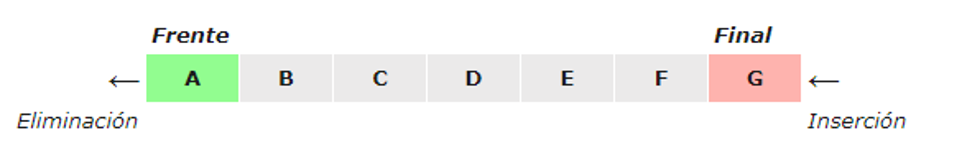
\includegraphics[width=5cm, height=2cm]{colas.png}
	\end{center}
	
	
	\subsection{Tipos : }
	
	\begin{itemize}
		\item \textbf{Colas circulares (anillos):}En las que el último elemento y el primero están unidos. \\
		
		\item \textbf{Colas de prioridad :}En ellas, los elementos se atienden en el orden indicado por una prioridad asociada a cada uno. Si varios elementos tienen la misma prioridad, se atenderán de modo convencional según la posición que ocupen. \\
		
		Hay 2 formas de implementación: 
		\begin{enumerate}
			\item Añadir un campo a cada nodo con su prioridad. Resulta conveniente mantener la cola ordenada por orden de prioridad. 
			\item Crear tantas colas como prioridades haya, y almacenar cada elemento en su cola. 
		\end{enumerate}
		\item \textbf{Bicolas :}Son colas en donde los nodos se pueden añadir y quitar por ambos extremos; se les llama DEQUE (Double Ended QUEue). Para representar las bicolas lo podemos hacer con un array circular con Inicio y Fin que apunten a cada uno de los extremos. 
		\begin{enumerate}
			\item \textbf{Bicolas de entrada restringida:}Son aquellas donde la inserción sólo se hace por el final, aunque podemos eliminar al inicio ó al final. 
			\item \textbf{Bicolas de salida restringida:}Son aquellas donde sólo se elimina por el final, aunque se puede insertar al inicio y al final.
		\end{enumerate}
		
	\end{itemize}
	
	
	\subsection{Desarrollo}
	
	\begin{itemize}
		\item \textbf{Estructura del programa.}
		
		\begin{center}
			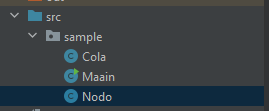
\includegraphics[width=5cm, height=2cm]{img1.png}
		\end{center}
		
		\begin{center}
			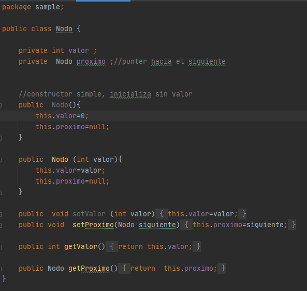
\includegraphics[width=5cm, height=6cm]{img2.png}
		\end{center}
		
		\begin{center}
			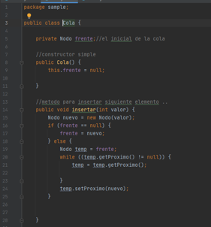
\includegraphics[width=5cm, height=6cm]{img3.png}
		\end{center}
		
		\begin{center}
			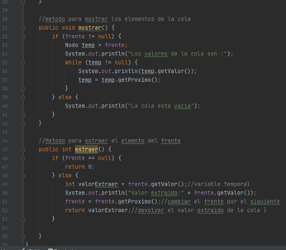
\includegraphics[width=5cm, height=6cm]{img4.png}
		\end{center}
		
		\begin{center}
			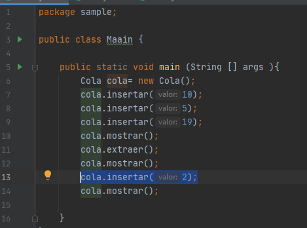
\includegraphics[width=5cm, height=5cm]{img5.png}
		\end{center}
		
		
		
		\item \textbf{Ventajas.}
		
		
		\begin{enumerate}
			\item No es preciso conocer la cantidad de elementos en tiempo de compilación. 
			\item Ni las inserciones ni las eliminaciones implican realizar corrimientos de los elementos de la lista. 
			\item Al utilizar una cola, sencillamente nos aseguramos que se procesan los dígitos en orden inverso; el primero en entrar en el primero en salir. 
			\item La implementación del TAD Cola con una lista enlazada permite ajustarse exactamente al número de elementos de la cola. utiliza dos apuntadores (referencias) para acceder a la lista. 
		\end{enumerate}
		
		\item \textbf{Desventajas.}
		
		\begin{enumerate}
			\item No permite el acceso directo a un elemento arbitrario de la lista. Para acceder al i-esimo elemento, debemos recorrer la lista, comenzando por el primer nodo, hasta llegar al elemento deseado. 
			\item Al asignar el arreglo en tiempo de compilación debe establecerse un límite a priori sobre el número de elementos que pueden ser almacenados en las listas. 
			\item La utilización de arrays tiene el problema de que la cola no pueda crecer indefinidamente, está limitada por el tamaño del array 
		\end{enumerate}
		
		
		\item \textbf{Implementación de la estructura de cola.}
		
		De manera similar a las pilas, las colas definen una estructura no estándar, de manera que se debe crear un nuevo tipo de dado, el tipo cola, que debe tener los siguientes elementos: \\
		
		\begin{itemize}
			\item Un arreglo de n elementos de algún tipo específico, puede incluso ser un tipo estándar o no. 
			\item Un número que indica el elemento que está en la posición del frente de la cola. 
			\item Un número que indica el elemento que está en la posición trasera de la cola.
		\end{itemize}
		
		Suponiendo que los elementos son números enteros, una idea para representar una cola es usar un arreglo para contener los elementos y emplear otras dos variables para representar la parte frontal y trasera de la cola.\\
		
	\end{itemize}
	
	
	\section{Conclusiones }
	
	\begin{itemize}
		\item Las colas circulares son una manera eficiente de aprovechar el espacio disponible, que muchas veces no se puede utilizar en las colas lineales. 
		\item Estan diseñadas para devolver los elementos ordenador tal como llegan. Para esto, las colas poseen un punto de acceso y otro de salida que logicamete estas son ubicados en extremos opuestos. Siempre vemos el elemento que esta primero o al frente.
	\end{itemize}
	
	
	
	% Bibliografia.
	%-----------------------------------------------------------------
	

	\section{Bibliografia}
	
	\bibliography{bibliografia}
	https://histinf.blogs.upv.es/2011/01/04/historia-de-las-bases-de-datos/ 
	http://virtual.usalesiana.edu.bo/web/conte/archivos/282.pdf 

	https://elibro.net/es/ereader/bibliotecaupt/50123?page=6
	https://elibro.net/es/lc/bibliotecaupt/titulos/50117
	http://ccc.inaoep.mx/ingreso/programacion/corto2015/Curso-PROPE-PyED-5-Pilas-Colas.pdf
\end{document}
